\documentclass{article}
\usepackage{microtype}
\usepackage{graphicx}
\usepackage{booktabs}
\usepackage{needspace}
\usepackage[hyperfootnotes=false]{hyperref}
\usepackage{xurl}
\newcommand{\theHalgorithm}{\arabic{algorithm}}
\usepackage[preprint]{icml2026}
\usepackage{amsmath,amssymb,amsthm,mathtools}
\usepackage{algorithm,algorithmic}
\usepackage{tikz}
\usepackage{pgfplots}
\usetikzlibrary{arrows.meta,positioning,calc,shapes.geometric,fit,backgrounds}
\pgfplotsset{compat=1.18}
% Okabe--Ito colors; labels and line styles also encode meaning.
\definecolor{scBlue}{HTML}{0072B2}
\definecolor{scOrange}{HTML}{E69F00}
\definecolor{scGreen}{HTML}{009E73}
\definecolor{scInk}{HTML}{263238}
\definecolor{scGray}{HTML}{6B747A}
\tikzset{
  scArrow/.style={-{Latex[length=1.5mm]},line width=0.65pt,draw=scGray},
  scSummary/.style={draw=scBlue,fill=scBlue!9,rounded corners=1.5pt,
    line width=0.85pt,font=\sffamily\fontsize{8}{9}\selectfont,
    inner sep=4pt,minimum width=11mm,text=scInk,align=center},
  scExact/.style={scSummary,draw=scGreen,fill=scGreen!12},
  scSplit/.style={scSummary,draw=scGray!60,fill=white,text=scGray,
    dashed,line width=0.55pt},
  scText/.style={font=\sffamily\fontsize{8}{9.5}\selectfont,text=scInk},
  scSmall/.style={font=\sffamily\fontsize{7}{8}\selectfont,text=scGray}
}

\usepackage[capitalize,noabbrev]{cleveref}
\theoremstyle{plain}
\newtheorem{theorem}{Theorem}
\newtheorem{lemma}[theorem]{Lemma}
\newtheorem{proposition}[theorem]{Proposition}
\newtheorem{corollary}[theorem]{Corollary}
\theoremstyle{definition}
\newtheorem{definition}[theorem]{Definition}
\theoremstyle{remark}
\newtheorem{remark}[theorem]{Remark}
\newcommand{\R}{\mathbb R}
\newcommand{\Q}{\mathbb Q}
\newcommand{\N}{\mathbb N}
\newcommand{\BF}{\operatorname{BF16}}
\newcommand{\RNE}{\operatorname{RNE}}
\newcommand{\E}{E_{24}}
\newcommand{\abs}[1]{\left|#1\right|}
\newcommand{\floor}[1]{\left\lfloor#1\right\rfloor}
\newcommand{\ceil}[1]{\left\lceil#1\right\rceil}
\newcommand{\raw}{\operatorname{raw}}
\newcommand{\sgn}{\operatorname{sgn}}
\newcommand{\profile}{\texttt{RATIONAL\_BF16\_V1}}
\newcommand{\code}[1]{\texttt{\small #1}}
% Generated by render_results.py; do not hand-edit.
\newcommand{\WriteAccepts}{7}
\newcommand{\WriteSteps}{96}

\icmltitlerunning{StateCut: Residual Attention Predicates and Exact Persistent Writes}
\icmlkeywords{attention, exact computation, interval arithmetic, formal verification, decoding}
\date{September 5, 2026}
\pdfstringdefDisableCommands{\def\\{ }}
\hypersetup{pdfsubject={Private research draft in ICML 2026 preprint format}}
% Contact is a name only; no private or invented email is embedded.
\makeatletter
\def\icmlcorrespondingauthor@text{Samuel Mausberg}
\makeatother

\begin{document}
\twocolumn[
\icmltitle{StateCut: Residual Attention Predicates\\and Exact Persistent Writes}
\begin{icmlauthorlist}
\icmlauthor{Samuel Mausberg}{statecut}
\end{icmlauthorlist}
\icmlaffiliation{statecut}{StateCut Project}
\vskip 0.3in
]
\printAffiliationsAndNotice{Research draft, not a conference submission.}

\begin{abstract}
Can a deterministic decoder certify its next transition without rereading
every historical key and value? We study sufficient conditions for preserving
both the emitted token and every persistent write under an explicit numerical
reference. The verifier evaluates signed attention residuals at rounding-cell
boundaries, using mergeable count, sum, and range summaries; a sharp refinement
retains the integer number of rows in the classical convex moment bound.
A persistent forest supports adaptive refinement, while a transactional
interval interpreter can certify persistent writes even when transient
activations remain uncertain. We prove the residual, rounding, partition, and
future-trace implications, and give a nonconstant family with zero raw-row
reads after preprocessing. The finite-count refinement certifies a case that
the chord rejects. On two pretrained checkpoints, sampled filtered heads match
dense E24 through fallback, while no captured attention call is certified in
full. Measured E24/backend differences and explicit formal-proof boundaries
leave deployed backend equivalence and end-to-end acceleration open.
\end{abstract}

\section{Introduction}
\label{sec:introduction}

During autoregressive decoding, historical key/value (KV) data are repeatedly
read to compute attention. Query-dependent sparse methods reduce those reads
by selecting a subset of the cache, with empirical quality evaluations
\citep{tang2024quest,ribar2024sparq}. We investigate a stricter contract:
skip historical reads only when a verifier establishes the exact reference
transition. Matching the current greedy token is insufficient because a small
change to a new KV entry can affect later tokens. Consequently, the certificate
must cover the persistent state as well as the immediate decision.

StateCut combines three ideas. First, it tests the residual $N-tD$ directly at
an output rounding boundary $t$, preserving dependence between an attention
numerator $N$ and denominator $D$. Second, an append-only forest makes root
summaries available without a compulsory scan of every fixed-size block.
Third, it accepts a speculative computation when every live persistent write
and the terminal greedy decision are exact. A failed attempt executes the
reference from the original state.

The mathematical ingredients have substantial antecedents. Adaptive exact
predicates are classical \citep{shewchuk1997}; the first-moment chord bound is
the Edmundson--Madansky inequality \citep{edmundson1957,madansky1959}; and
neural-network interval propagation is an established verification method
\citep{singh2019deeppoly}. We specialize and compose these ingredients for
attention and persistent decoder state. We also derive and implement an exact
finite-cardinality version of the moment envelope. This improves the previous
continuous-mass relaxation without adding summary fields. We make no priority
claim for the underlying convex extremal argument.

The executable target is a rational arithmetic profile with correctly rounded
BF16 materializations. This choice makes algebraic reassociation legitimate
and gives a small reference implementation against which to test certificates.
It does not identify that profile with PyTorch, FlashAttention, or a pretrained
checkpoint's instruction-level behavior. Our contribution is a sufficient
certificate and a falsifiable research artifact, with the remaining numerical
and systems obligations stated explicitly.

\section{Contract and Numerical Reference}
\label{sec:contract}

\begin{figure*}[t]
\centering
\begin{minipage}[t]{0.49\textwidth}\centering\vspace{0pt}
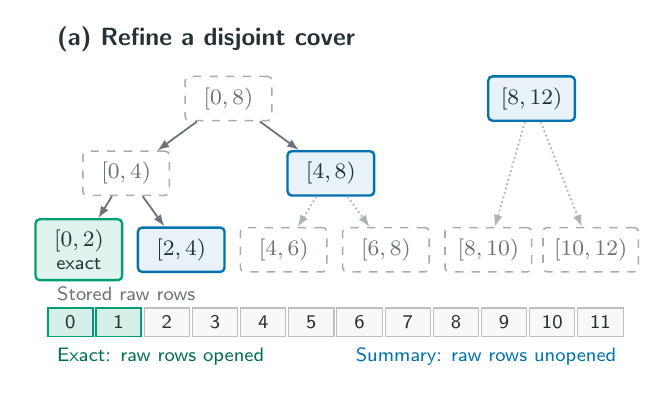
\begin{tikzpicture}[x=1cm,y=1cm]
\path[use as bounding box] (-.25,-.5) rectangle (7.5,4.05);
\node[scText,anchor=west,font=\sffamily\bfseries\small] at (0,3.9)
  {(a) Refine a disjoint cover};
\node[scSplit] (r0) at (2.3,3.15) {$[0,8)$};
\node[scSummary] (r1) at (6.15,3.15) {$[8,12)$};
\node[scSplit] (c0) at (1.0,2.2) {$[0,4)$};
\node[scSummary] (c1) at (3.6,2.2) {$[4,8)$};
\node[scExact] (l0) at (0.4,1.23) {$[0,2)$\\[-1pt]{\scriptsize exact}};
\node[scSummary] (l1) at (1.7,1.23) {$[2,4)$};
\node[scSplit] (l2) at (3.0,1.23) {$[4,6)$};
\node[scSplit] (l3) at (4.3,1.23) {$[6,8)$};
\node[scSplit] (l4) at (5.6,1.23) {$[8,10)$};
\node[scSplit] (l5) at (6.9,1.23) {$[10,12)$};
\foreach \from/\to in {r0/c0,r0/c1,c0/l0,c0/l1}
  \draw[scArrow] (\from) -- (\to);
\foreach \from/\to in {c1/l2,c1/l3,r1/l4,r1/l5}
  \draw[scArrow,densely dotted,draw=scGray!55] (\from) -- (\to);
\node[scSmall,anchor=west] at (0,0.67) {Stored raw rows};
\foreach \x in {0,...,11}{
  \pgfmathsetmacro{\left}{0.005+0.612*\x}
  \ifnum\x<2
    \draw[draw=scGreen,fill=scGreen!16,line width=.6pt]
       (\left,0.13) rectangle ++(.575,.36);
  \else
    \draw[draw=scGray!45,fill=scGray!5,line width=.4pt]
       (\left,0.13) rectangle ++(.575,.36);
  \fi
  \node[scSmall,text=scInk] at (\left+.2875,.31) {\x};
}
\node[scSmall,anchor=west,text=scGreen!70!black] at (0,-.13) {Exact: raw rows opened};
\node[scSmall,anchor=east,text=scBlue] at (7.35,-.13) {Summary: raw rows unopened};
\end{tikzpicture}

\end{minipage}\hfill
\begin{minipage}[t]{0.49\textwidth}\centering\vspace{0pt}
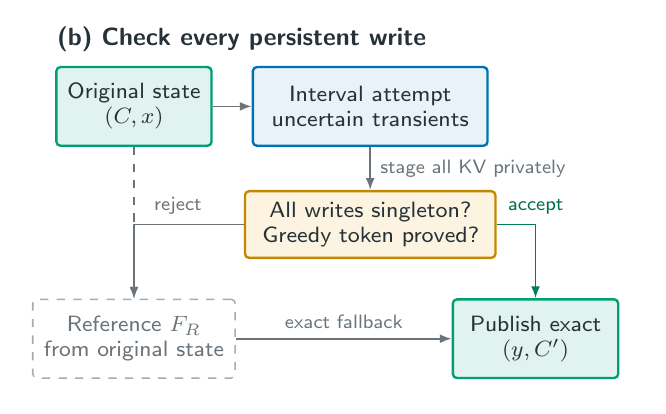
\begin{tikzpicture}[x=1cm,y=1cm]
\path[use as bounding box] (-.25,-.5) rectangle (7.5,4.05);
\node[scText,anchor=west,font=\sffamily\bfseries\small] at (0,3.9)
  {(b) Check every persistent write};
\node[scExact,minimum width=18mm,minimum height=10mm] (old) at (1.1,3.05)
  {Original state\\$(C,x)$};
\node[scSummary,text width=27mm,minimum height=10mm] (attempt) at (4.1,3.05)
  {Interval attempt\\uncertain transients};
\node[scSummary,draw=scOrange!85!black,fill=scOrange!12,
  text width=29mm,minimum height=8mm] (gate) at (4.1,1.55)
  {All writes singleton?\\Greedy token proved?};
\node[scSplit,minimum width=20mm,minimum height=10mm] (dense) at (1.1,.1)
  {Reference $F_R$\\from original state};
\node[scExact,minimum width=21mm,minimum height=10mm] (commit) at (6.2,.1)
  {Publish exact\\$(y,C')$};
\draw[scArrow] (old) -- (attempt);
\draw[scArrow] (attempt) -- node[right,scSmall] {stage all KV privately} (gate);
\draw[scArrow,dashed] (old.south) -- (dense.north);
\draw[scArrow] (gate.west) -| node[pos=.3,above,scSmall] {reject} (dense.north);
\draw[scArrow,draw=scGreen!80!black] (gate.east) -|
  node[pos=.3,above,xshift=2mm,scSmall,text=scGreen!70!black] {accept} (commit.north);
\draw[scArrow] (dense.east) -- node[above,scSmall] {exact fallback} (commit.west);
\end{tikzpicture}

\end{minipage}
\caption{StateCut's two boundaries. Left: a query refines only part of a
persistent forest. Solid nodes form the current disjoint frontier; opening
$[0,2)$ reads two raw rows, while the other solid nodes retain summary
enclosures. Dashed nodes are outside the current frontier. Right: uncertain
transients remain private until every persistent write and the terminal
decision are proved exact. Rejection invokes the reference on the original
state. Colors are redundant with node labels and line styles.}
\label{fig:architecture}
\end{figure*}

Fix model parameters, operator semantics, legal inputs, visibility rules, and
the tie rule. Let
\begin{equation}
 F_R(C,x)=(y,C')
 \label{eq:transition}
\end{equation}
process a pending token $x$, return the predicted token $y$, and produce the
state $C'$. The state contains every object that can influence a future
invocation. In the prototype it includes the model identity, per-layer exact
KV, token prefix, and position. A serving implementation additionally needs
the relevant masks, position conventions, branch identity, slot ownership,
generations, synchronization, and any recurrent or mutable state. These
fields are part of the contract when they are live; a KV-only theorem cannot
justify omitting them.

\paragraph{Why token equality is weaker.}
Consider $F(s)=(\mathbf 1[s<0],s-1/2)$. States $s=1/4$ and $s=3/4$ return
the same first token. Their successors have different signs, so the next
tokens differ. In contrast, equality of \emph{both} outputs of
\cref{eq:transition} composes by induction. Sampling would require its own
coupling argument and an inventory of random state; the present policy is
greedy with the smallest vocabulary index winning a tie.

\paragraph{Arithmetic profile.}
For rational scores, define
\begin{equation}
 \begin{gathered}
 \E(z)=2^{-24}\RNE_{\mathbb Z}(2^{24}e^z),\\
 w_i=\E(q^\top k_i),\qquad
 A_j=\frac{\sum_i w_i v_{ij}}{\sum_i w_i}.
 \end{gathered}
 \label{eq:profile}
\end{equation}
The query includes the exact attention scale. Dot products and reductions
are rational; the materialization is $\BF(A_j)$ with nearest-even rounding.
The profile canonicalizes signed zero and rejects nonfinite results. The
exponential oracle refines rigorous Taylor enclosures until integer rounding
is decided, with explicit resource limits and rejection on exhaustion.
Weights can round to zero, so denominator positivity is a separate
obligation. Matrix products sum exactly before each prescribed rounding cut.
RMS normalization uses $\epsilon=1/256$, and the gate is the specified
$\BF(x/(1+\E(-x)))$. The full graph is defined by
\code{src/statecut/model.py} and \code{docs/REFERENCE.md}.

We call this profile \profile{}. It is a deliberately explicit numerical
object, not a claim of bitwise agreement with a common backend. In
particular, $\E$ is not invariant under a common score shift: quantizing
exponentials changes their ratios. PyTorch documents that algebraically
equivalent reductions can produce different floating-point results
\citep{pytorchaccuracy}. A mathematical softmax proof therefore needs a
separate bridge before it can replace a pinned GPU instruction graph.

\section{Residual Certificates from Mergeable Moments}
\label{sec:residual}

A summary of $n>0$ rows stores coordinatewise key minima and maxima and,
for each value coordinate,
\begin{equation}
 S=\sum_{i=1}^n v_i,\qquad \ell\le v_i\le u.
 \label{eq:summary}
\end{equation}
The builder uses actual extrema; the theorem only requires valid bounds.
Counts and sums add under merging, and extrema take minima and maxima.
The reference also retains positive and negative moments for an independent
interval intersection. No query-time raw scan is needed to merge summaries.
Summaries must belong to the actual visible rows and the correct layer/head.
Trusted construction is a premise, not a consequence of shape validation.

Interval dot products give $q^\top k_i\in[L,U]$ throughout a node. Since
$\E$ is monotone, $a=\E(L)\le w_i\le\E(U)=b$.
The same reasoning allows interval queries containing their reference
values. Unsupported masks, biases, or visibility rules require additional
sound score bounds; they are not implicitly covered.

For one value coordinate and threshold $t$, write
\begin{equation}
 \begin{gathered}
 D=\sum_iw_i,\qquad N=\sum_iw_iv_i,\\
 R(t)=N-tD=\sum_iw_i(v_i-t),
 \end{gathered}
 \label{eq:residual}
\end{equation}
and set $m=(a+b)/2$, $h=(b-a)/2$.

\Needspace{5\baselineskip}
\begin{lemma}[Residual from an absolute-sum envelope]
\label{lem:generic}
If $a\le w_i\le b$ and $\sum_i|v_i-t|\le C(t)$, then
\begin{equation}
 m(S-nt)-hC(t)\le R(t)\le m(S-nt)+hC(t).
 \label{eq:bound}
\end{equation}
\end{lemma}
\begin{proof}
Subtract $m(S-nt)$ from \cref{eq:residual}. The result is
$\sum_i(w_i-m)(v_i-t)$, whose absolute value is at most
$h\sum_i|v_i-t|$ by $|w_i-m|\le h$ and the triangle inequality.
\end{proof}

\subsection{The Classical Chord Envelope}

Convexity of $v\mapsto|v-t|$ gives, for $\ell<u$,
\begin{equation}
 C_{\rm ch}(t)=
 \frac{(nu-S)|\ell-t|+(S-n\ell)|u-t|}{u-\ell}.
 \label{eq:chord}
\end{equation}
For $\ell=u$, put $C_{\rm ch}(t)=n|\ell-t|$. Then
$\sum_i|v_i-t|\le C_{\rm ch}(t)$. This is the univariate
Edmundson--Madansky first-moment bound applied to the empirical distribution
\citep{edmundson1957,madansky1959}; \cref{app:chord} gives the proof.
It is sharp when arbitrary real mass is allowed at the two endpoints,
although those masses need not correspond to integer row counts.

Both $S-nt$ and \cref{eq:chord} are unchanged by
$(v_i,t)\mapsto(v_i+c,t+c)$. Thus a large common value offset does not
itself enlarge the residual uncertainty. An independent quotient enclosure
usually loses that cancellation.

\subsection{A Sharp Envelope for an Integer Number of Rows}
\label{sec:integer}

The continuous-mass relaxation discards information already present in the
integer count $n$. Retaining it gives a stronger bound at constant summary
cost. For $d=u-\ell>0$, define
\begin{equation}
 r=\frac{S-n\ell}{d},\qquad k=\floor{r},\qquad
 x_* =\ell+(r-k)d.
 \label{eq:integerparams}
\end{equation}
Here $0\le r\le n$. If $k<n$, put
\begin{equation}
 C_{\rm int}(t)=k|u-t|+(n-k-1)|\ell-t|+|x_*-t|.
 \label{eq:integer}
\end{equation}
If $k=n$, use $C_{\rm int}(t)=n|u-t|$; the case $d=0$ uses
$n|\ell-t|$.

\begin{theorem}[Sharp finite-cardinality envelope]
\label{thm:integer}
For integer $n\ge1$ and feasible $(S,\ell,u)$,
\begin{equation}
 \max_{\substack{v\in[\ell,u]^n\\\sum_i v_i=S}}
       \sum_i|v_i-t|=C_{\rm int}(t)\le C_{\rm ch}(t).
 \label{eq:sharp}
\end{equation}
Consequently, \cref{eq:bound} with $C_{\rm int}$ gives the exact minimum
and maximum of $R(t)$ over this value set and all independent choices
$w_i\in[a,b]$.
\end{theorem}
\begin{proof}
If two coordinates are interior, preserve their sum and vary them in
opposite directions. Their contribution to the objective is convex in that
variation. One endpoint of its feasible interval has at least the original
objective value and puts at least one coordinate at $\ell$ or $u$.
Repeating leaves at most one interior coordinate. The fixed sum forces the
endpoint counts and remaining value in \cref{eq:integerparams,eq:integer}.
This construction attains $C_{\rm int}$, and the chord bound applied to it
proves the inequality. Choosing
$w_i=m\pm h\sgn(v_i-t)$ attains the two residual endpoints.
\cref{app:integer} details boundary cases and termination.
\end{proof}

The sharpness is for the stated boxed relaxation. It does not retain
key/value correlations, individual score constraints, discrete BF16 value
feasibility, or discrete $\E$ weight feasibility. Those restrictions can
make the true attention range smaller. For rational summary inputs, the
extremal value vector is rational, so no irrational values are needed.

The refinement is translation invariant and never weaker than the chord
bound. Its additive benefit is bounded:
\begin{equation}
 0\le C_{\rm ch}(t)-C_{\rm int}(t)\le (u-\ell)/2.
 \label{eq:improvement}
\end{equation}
Thus the improvement per residual endpoint is at most $h(u-\ell)/2$;
there is no implied factor improvement as $n$ grows. For $n=3$, $S=48$,
$\ell=63/4$, and $u=65/4$, the difference is strict at most interior
thresholds (\cref{fig:envelope}).

\begin{figure}[t]
\centering
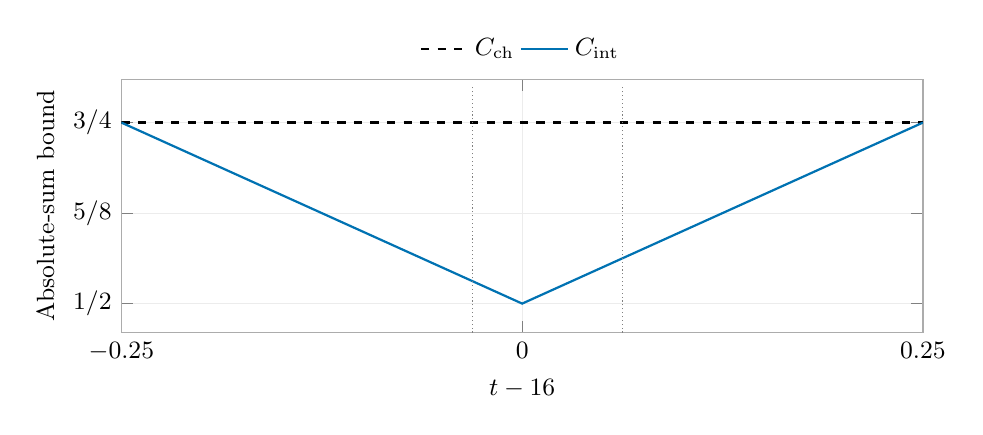
\begin{tikzpicture}
\begin{axis}[
  width=0.97\columnwidth,height=4.8cm,
  xlabel={$t-16$},ylabel={Absolute-sum bound},
  xmin=-0.25,xmax=0.25,ymin=0.46,ymax=0.81,
  xtick={-0.25,0,0.25},ytick={0.5,0.625,0.75},
  yticklabels={$1/2$,$5/8$,$3/4$},
  tick label style={font=\small},label style={font=\small},
  legend style={font=\small,at={(0.5,1.03)},anchor=south,
                legend columns=2,draw=none},
  grid=major,grid style={gray!15},
  axis line style={gray!65}]
\addplot[black,dashed,thick,domain=-0.25:0.25,samples=2]{0.75};
\addlegendentry{$C_{\rm ch}$}
\addplot[scBlue,thick] coordinates {(-0.25,0.75) (0,0.5) (0.25,0.75)};
\addlegendentry{$C_{\rm int}$}
\addplot[gray,densely dotted,forget plot] coordinates {(-0.03125,0.46) (-0.03125,0.8)};
\addplot[gray,densely dotted,forget plot] coordinates {(0.0625,0.46) (0.0625,0.8)};
\end{axis}
\end{tikzpicture}

\caption{Exact analytic envelopes for three rows with sum $48$ and range
$[63/4,65/4]$. The integer count forces the extremal vector
$(63/4,16,65/4)$; a continuous-mass relaxation permits $1.5$ rows at each
endpoint. The vertical marks are the two BF16 boundaries of $16$.
This plot is a theorem illustration, not measured model data.}
\label{fig:envelope}
\end{figure}

\subsection{Safe Intersections}

Let $P=\sum_i\max(v_i,0)$ and $M=\sum_i\min(v_i,0)$. Then
$N\in[aP+bM,bP+aM]$ and $D\in[na,nb]$. Interval subtraction
of $tD$ gives another residual enclosure. Intersecting it with
\cref{eq:bound} is sound. A disjoint intersection signals a violated
arithmetic or provenance premise and must reject. The direct threshold
predicate itself requires no division by an uncertain denominator; computing
the moment parameters still uses scalar divisions by known summary values.

\section{From Residual Signs to Exact Decisions}
\label{sec:gates}

For a proposed finite output $y$, let $J_y$ be its exact rounding cell, with
boundaries $t_-$ and $t_+$ and separately specified endpoint inclusion.
Ordinary BF16 nearest-even cells include both midpoints for even
significands and exclude both for odd significands. The canonical zero cell
is $[-2^{-134},2^{-134}]$; maximal finite values have an open overflow
boundary. Neighbor spacing can be asymmetric at powers of two.

\begin{theorem}[Residual rounding gate]
\label{thm:gate}
Suppose $D>0$. Let $\underline R(t_-)$ and $\overline R(t_+)$ be sound
lower and upper residual bounds. If
\begin{equation}
 \underline R(t_-)\ge0,\qquad \overline R(t_+)\le0,
 \label{eq:gate}
\end{equation}
with a strict comparison at each excluded endpoint, then $\BF(N/D)=y$.
\end{theorem}
\begin{proof}
The identity $R(t)=D(N/D-t)$ and $D>0$ convert each residual sign to
the corresponding cell-membership inequality. Membership in $J_y$ is
precisely the definition of rounding to $y$.
\end{proof}

For a disjoint frontier of nodes, sum residual bounds at the \emph{same}
threshold. An opened leaf contributes its exact $N-tD$. The proposal is
untrusted: a bad candidate may cause rejection, but cannot create a false
certificate under the stated premises. The reference proposer uses midpoint
weights and summary means; its work is charged to the filter.

A centered quotient $t+R(t)/D$ is sound when denominator division is valid,
and is useful for propagating transient intervals. It can nevertheless
remain too wide: its independently combined extrema need not be jointly
attainable. The sign checks in \cref{eq:gate} retain the dependence needed
for rounding without constructing that quotient.

\begin{proposition}[Nonconstant family with no raw reads]
\label{prop:family}
Let $n>0$ be even, with half the values $63/4$ and half $65/4$. For any
weights in $[7/8,9/8]$, $\BF(N/D)=16$, and the chord residual gate proves
this from one summary.
\end{proposition}
\begin{proof}
Here $S=16n$, $m=1$, and $h=1/8$. The cell of $16$ is the closed,
asymmetric interval $[511/32,257/16]$. Both boundaries are inside the
value range and $C_{\rm ch}=n/4$ there. The lower-bound residual is
$n/32-n/32=0$ at the left endpoint; the upper-bound residual is
$-n/16+n/32=-n/32<0$ at the right. Finally $D\ge7n/8>0$.
\end{proof}

This is an existence result after preprocessing. The illustrative weight
box is not the same as the $\E(\pm1/8)$ box in the executable balanced
fixture. That fixture is separately checked against its actual quantized
weights. No acceptance rate for pretrained activations follows from either
construction.

\section{A Persistent Refinement Forest}
\label{sec:forest}

Raw leaves contain at most $B$ consecutive entries. Every full leaf is
sealed and merged with adjacent equal-rank roots, as in a binary counter.
A partial tail is separate. For $m=\floor{N/B}$ full leaves there are
$\operatorname{popcount}(m)$ completed roots and at most one tail, hence
$O(\log(2+N/B))$ initial summaries. Raw entries are retained; the index
does not establish memory compression.
\Cref{fig:architecture} illustrates a partially refined frontier.

\begin{algorithm}[t]
\caption{Exact attention cut from a disjoint frontier}
\label{alg:attention}
\begin{algorithmic}[1]
\REQUIRE Trusted forest, query $q$, expansion budget $K$
\STATE $\mathcal F\leftarrow$ roots and tail; all pieces unresolved
\FOR{$s=0,\ldots,K$}
  \STATE Bound each unresolved piece's weights; propose $y$
  \STATE Sum denominator and residual bounds over $\mathcal F$
  \IF{denominator is positive and every coordinate passes
       \cref{thm:gate}}
    \STATE \textbf{return} $y$ with an accepted-cut certificate
  \ENDIF
  \IF{$s=K$ or no unresolved pieces remain}
    \STATE \textbf{break}
  \ENDIF
  \STATE Choose an unresolved piece using enclosure width
  \IF{it is internal}
    \STATE Replace it by its two children
  \ELSE
    \STATE Read its raw rows and store its exact contribution
  \ENDIF
\ENDFOR
\STATE Exactify only unresolved pieces; reuse exact contributions
\STATE \textbf{return} exactly rounded dense attention under \profile{}
\end{algorithmic}
\end{algorithm}

\begin{theorem}[Partition and raw-read accounting]
\label{thm:frontier}
The frontier in \cref{alg:attention} remains a disjoint cover of the
visible prefix. Each raw leaf is read at most once, including exploration
and fallback, under the exact-rational reference.
\end{theorem}
\begin{proof}
Append and adjacent binary carries preserve consecutive disjoint coverage.
A split replaces $[a,c)$ by $[a,b)$ and $[b,c)$ with the same union.
Exactification changes only representation. Exact pieces are never opened
again, and fallback descends only through unresolved pieces; those cannot
overlap exact ones. Thus no raw leaf is read twice.
\end{proof}

A root-only attempt requires
$O((d_k+d_v)\log(2+N/B))$ scalar summary work, and
$O(d_k+d_v)$ for a single root. This is a logical operation count;
rational bit complexity, allocation, and interpreter overhead are outside
that count. The current Python scheduler scans the frontier for priority
on each expansion. The tree can still be fully explored, followed by all
raw reads; a budget limits speculative exploration, not fallback work.

Across $m$ completed leaves, fewer than $m$ binary merges occur, so merges
are amortized constant per completed leaf. Summary updates and initial
construction must still be charged. Python root tuples and the toy token
prefix are copied, with the latter costing $O(T)$ per append. A backend
that fixes a nonassociative reduction tree may require a fresh dense pass
after failed speculation; \cref{thm:frontier} does not remove that cost.

\section{Certifying the Persistent Write Frontier}
\label{sec:writes}

Some consumers erase transient uncertainty. Let $W(h)$ denote every new
persistent write and $G(h)$ the terminal decision. It is sufficient to prove
$W(\hat h)=W(h_R)$ and $G(\hat h)=G(h_R)$ even when
$\hat h\ne h_R$. StateCut's \code{writes} strategy realizes this
observation using a sound interval interpreter, exact rounding, and private
staging. It requires singleton rounded K/V coordinates before appending to
a staged forest; queries and attention outputs may remain intervals.
The \code{cuts} strategy instead certifies exact attention
materializations and executes the exact suffix, using a decision gate only
where no later persistent writes depend on uncertain transients.

\begin{lemma}[Greedy decision with ties]
\label{lem:argmax}
Suppose $z_j\in[L_j,U_j]$. Candidate $c$ is the smallest-index maximizer if
\begin{equation}
 U_j<L_c\ (j<c),\qquad U_j\le L_c\ (j>c).
 \label{eq:argmax}
\end{equation}
\end{lemma}
\begin{proof}
For an earlier competitor, $z_j\le U_j<L_c\le z_c$; for a later
competitor, $z_j\le U_j\le L_c\le z_c$. These are exactly the required
strict and weak comparisons.
\end{proof}

\begin{theorem}[Exact transition and future traces]
\label{thm:state}
Assume every represented interval contains its reference intermediate,
every newly persistent scalar has a singleton interval, and the full
vocabulary satisfies \cref{eq:argmax}. Commit all staged writes together.
The resulting pair $(y,C')$ equals \cref{eq:transition}. If every rejected
attempt runs $F_R$ from the original state, the filtered decoder has the
same tokens and persistent state for every finite legal continuation.
\end{theorem}
\begin{proof}
A reference write contained in $[a,a]$ equals $a$ by antisymmetry.
Coordinatewise equality covers every new persistent write; unchanged
committed fields remain equal. \Cref{lem:argmax} proves token equality.
An accepted step and a rejected step therefore both equal $F_R$. Induct
over supplied input tokens. For autonomous decoding, use state $(C,x)$
and feed the common output $y$ as the next pending input.
\end{proof}

The interpreter uses signed interval affine operations, sound interval
squaring and square roots, and monotone BF16 rounding. It multiplies an
interval for $x$ by an interval for $1/(1+\E(-x))$; it does not assume
the entire SiLU-like function is monotone. Positive RMS epsilon prevents a
zero normalizer. \Cref{app:interpreter} explains the containment induction
and its trusted components. Any ambiguous write or decision, invalid
denominator, or resource failure discards the attempted transition before
dense fallback. There is no partial commit or future repair debt.

\section{Evaluation and Evidence Scope}
\label{sec:evaluation}

We test three distinct questions: whether a predicate accepts fewer raw
reads while preserving the named reference, whether complete toy-decoder
states remain equal, and whether device or pretrained observations expose
obstacles to deployment. The first two use exact-rational oracles. Device
tests and pretrained captures are separately scoped in the generated
measurement record below. All tabulated logical-read data are read from
machine-readable experiment artifacts by \code{paper/render\_results.py}.

\subsection{Paired Logical-Read Ablations}

The balanced fixture uses repeated four-way combinations of keys
$\pm1/8$ and values $16\pm1/4$, query $q=1$, and leaves of $B=32$.
It compares the original independent numerator/denominator gate, a
centered-quotient tree gate, and the direct residual tree gate on identical
rows with zero expansion budget. Every result is checked against dense
\profile{}. \Cref{tab:reads} reports raw reads and summary reads at
four lengths. Index construction reads the entire prefix and is excluded
from query reads, not from total system cost.

% Generated by render_results.py; do not hand-edit.
\begin{table}[t]
\centering
\small
\caption{Balanced fixture: raw rows / summary records read per query. All three methods agree with dense E24. Initial indexing is additional work.}
\label{tab:reads}
\begin{tabular}{rccc}
\toprule
Rows & Indep. flat & Centered ratio & Direct \\
\midrule
128 & 128/4 & 128/1 & 0/1 \\
512 & 512/16 & 512/1 & 0/1 \\
2,048 & 2048/64 & 2048/1 & 0/1 \\
8,192 & 8192/256 & 8192/1 & 0/1 \\
\bottomrule
\end{tabular}
\end{table}


The direct gate accepts the balanced cases from one summary. Both divided
variants require dense fallback. This separates the threshold predicate
from merely centering a quotient, and the tree from the original flat
summary scan. A separately seeded unstructured case retains full raw
fallback; there is no universal sublinear claim.

\paragraph{Finite-cardinality improvement.}
For $n=3$, $S=48$, $\ell=63/4$, $u=65/4$, and score bounds
$[-3/20,3/20]$, the integer-count residual gate can pass the cell of $16$
where the chord residual gate fails. The experiment fixes the same summary,
proposal, and actual $\E$ weight endpoints for both bounds. Sharpness tests
enumerate small rational grids and endpoint weights, and include
translation, degeneracy, and exact-integer input cases.
% Generated by render_results.py; do not hand-edit.
The recorded lower-bound residuals at the left cell boundary are
\begin{equation}
\underline R_{\rm ch}=-\frac{4862889}{268435456}<0,\quad \underline R_{\rm int}=\frac{497277}{33554432}>0.
\end{equation}
Both methods return the dense result 16; the chord method reads 3 raw rows and the integer method reads 0. An exhaustive finite-grid audit checks 5,004 row multisets, 35,028 row/threshold combinations, and 1,218 fixed-sum/threshold optima against both attained residual extremes. It uses counts 1--6 and the nine-point grid from $-1$ to $1$ in increments of $1/4$; these finite tests support the implementation, while the general bound is proved mathematically.


\begin{figure}[t]
\centering
\begin{tikzpicture}
\begin{axis}[
  width=0.97\columnwidth,height=5.1cm,
  xlabel={Rows in summary (log scale)},ylabel={Raw rows read (\%)},
  xmode=log,log basis x=2,xmin=2.65,xmax=74,
  ymin=-8,ymax=112,ytick={0,50,100},
  xtick={3,5,9,17,33,65},xticklabels={3,5,9,17,33,65},
  tick label style={font=\small},label style={font=\small},
  legend style={font=\small,at={(0.5,1.03)},anchor=south,
    legend columns=1,draw=none},
  grid=major,grid style={gray!15},axis line style={scGray!70}]
\addplot[scInk,densely dashed,thick,mark=triangle*,mark size=2.4pt]
  table[x=rows,y=chord,col sep=comma] {generated/integer_ablation.csv};
\addlegendentry{Chord, both score ranges}
\addplot[scBlue,thick,mark=*,mark size=2.2pt]
  table[x=rows,y=integer013,col sep=comma] {generated/integer_ablation.csv};
\addlegendentry{Integer count, $|s|\le0.13$}
\addplot[scOrange!85!black,dashed,thick,mark=square*,mark size=2.1pt]
  table[x=rows,y=integer015,col sep=comma] {generated/integer_ablation.csv};
\addlegendentry{Integer count, $|s|\le0.15$}
\end{axis}
\end{tikzpicture}

\caption{Measured raw reads in the finite-count ablation. Each point is one
deterministic odd-length fixture with fixed score magnitude, zero expansion
budget, and a single summary. The chord gate reads all rows. Finite-count
gains disappear at larger counts, consistent with the additive bound in
\cref{eq:improvement}. Lines connect tested points, not a fitted model.}
\label{fig:integer-ablation}
\end{figure}
\Cref{fig:integer-ablation} retains both the favorable finite-count cases
and the cases where both methods fall back.

\subsection{Complete-State and Write-Frontier Checks}

Four small random decoders (seeds $0,1,8,19$) each generate 24 transitions
under both strategies, with expansion budget 3 and leaf size 4. The harness
compares every returned token and complete state to dense execution.
% Generated by render_results.py; do not hand-edit.
\begin{table}[t]
\centering
\small
\caption{Complete-state toy-decoder comparisons. Raw reads sum over layers and steps; write acceptance applies only to the writes strategy. Every compared token and full state agrees.}
\label{tab:state}
\begin{tabular}{lrrr}
\toprule
Strategy & Steps & Raw rows & Write accepts \\
\midrule
Cuts & 96 & 588 & --- \\
Writes & 96 & 2,254 & 7 \\
\bottomrule
\end{tabular}
\end{table}

These trajectories are deterministic constructed tests, not independent
samples from an LLM workload. The write-frontier acceptance rate is
\WriteAccepts{} of \WriteSteps{} steps; broad interval propagation
often fails. A separate two-layer construction permits a non-singleton
attention materialization yet certifies all persistent writes and the
decision without historical raw reads. Its second-layer K/V projections
are zero, so it establishes logical separation rather than typical model
behavior.

\subsection{Hardware, Pretrained Captures, and Formal Build}
\label{sec:measured}
% Generated by render_results.py; do not hand-edit.
The GH200 device arithmetic oracle check passed 68,851 comparisons: 2,500 moment cases, 65,279 finite canonical BF16 cells, 1,025 E24 weight cases, 42 lattice-rounding cases, and 5 negative-tail cases. These are executed finite comparisons, not a formal proof of device arithmetic. The CUDA checker uses the chord envelope; the finite-count refinement is used by the rational CPU reference.

On NVIDIA GH200 480GB (compute capability 9.0), a synthetic 8-head, 32,768-row, 64-coordinate root gate has a 62.85~$\mu$s median single-call event span (67.62~$\mu$s empirical 95th percentile), including host submission gaps. Graph batches of 100 sequential fixed-input calls give 45.84~$\mu$s median per call (45.85~$\mu$s 95th percentile); the separate SDPA primitive gives 32.27~$\mu$s in that graph protocol. Recorded construction took 144.68~ms. The proposal was the construction's known value 16, and the accepted gate read zero raw KV rows. Torch 2.7.0 and CUDA 12.8 were used. Graph amortization is not token latency. The two primitives have different numerical contracts; construction, refinement, and a decoder suffix are excluded from their event spans.

\begin{table}[t]
\centering
\small
\caption{Pretrained observer transparency, compared to the unchanged backend. State comparisons include prefill and every decode step; events are captured decode attention calls. This does not run a filtered replacement.}
\label{tab:pretrained}
\begin{tabular}{lrrrr}
\toprule
Model & Cases & Steps & States & Events \\
\midrule
Qwen2.5-0.5B & 6 & 18 & 24 & 432 \\
SmolLM2-135M & 6 & 18 & 24 & 540 \\
\bottomrule
\end{tabular}
\end{table}

The observer study uses pinned checkpoint revisions, three deterministic prompt constructions at contexts 128 and 512, and three decode steps per case. All recorded per-layer KV tensors agree bitwise and final-position logits agree in value with the unobserved run. It tests capture transparency; it does not test StateCut as a model replacement. Checkpoint hashes and exact prompt token IDs are retained in the source records.

% Generated by render_results.py; do not hand-edit.
\paragraph{Pretrained local-gate acceptance.}

The CUDA audit evaluates 972 captured attention calls and 10,908 query heads per configuration across both checkpoints. It compares a summary-mean proposal with the already observed SDPA output as a diagnostic oracle proposal. The oracle's dense computation is additional work, and its output need not equal E24.

\begin{table}[t]
\centering
\small
\caption{Pretrained CUDA acceptance: 10,908 heads and 972 calls per configuration. Mean uses the lattice enclosure. Oracle columns compare the half-quantum (HQ) and lattice (L) weight enclosures. The last column counts complete calls for mean/oracle with L.}
\label{tab:cudaacceptance}
\begin{tabular}{rcccc}
\toprule
Block & Mean & Oracle HQ & Oracle L & Calls \\
\midrule
1 & 0 & 254 & 280 & 0/0 \\
16 & 0 & 0 & 0 & 0/0 \\
64 & 0 & 0 & 0 & 0/0 \\
128 & 0 & 0 & 0 & 0/0 \\
\bottomrule
\end{tabular}
\end{table}

Monotone rounding of outward exponential endpoints onto the E24 lattice tightens the half-quantum enclosure (\cref{app:lattice}) and changes block-1 oracle acceptance from 254 to 280 heads. No complete all-head call passes. Block size 1 reads one summary per row, so its local certificates supply no sublinear summary-read advantage. Domain rejection and failure to prove positive mass are counted separately in \cref{app:domains}. These fixed workloads provide negative evidence for the current coarse summaries, not a population acceptance estimate.

% Generated by render_results.py; do not hand-edit.
\paragraph{Exact reference on captured heads.}
A deterministic subset evaluates 72 query heads (4,608 coordinates): the first two heads in the first, middle, and last layer at the first decode step for each model/prompt/context case. The finite-count CPU filter agrees with dense E24 on every tested head, using all raw rows through fallback in every case. E24 matches the observed SDPA bits on 4,107 coordinates and differs on 501. This comparison uses E24's canonical zero and the unmodified observed bits. The measured disagreement rules out treating these numerical profiles as interchangeable. One Qwen head has actual positive scores from 1,237.073 to 1,280.256; extending the rigorous CPU exponential oracle to 2,048 with magnitude-aware precision supports the tested cases. No common score shift is applied.


Capture-only evaluation preserves the selected backend's returned output
and records actual query, key, value, and output tensors. Re-evaluating
those tensors under \profile{} asks whether the profiles happened to
agree on the observed input. It cannot prove a universal numerical bridge,
and observing one attention layer cannot establish a complete decoder
transition. A CUDA gate microbenchmark measures the supplied local
certificate; its comparison to a separate SDPA primitive does not measure
an integrated decoder speedup.

% Generated by render_results.py; do not hand-edit.
The pinned Lean build succeeds and audits 66 source theorems (84 compiled theorem constants including generated helpers). Only the standard foundational axioms \code{propext}, \code{Classical.choice}, and \code{Quot.sound} occur. The compiled results cover chord and finite-count residual bounds, finite-count attainment and chord dominance, a mathematical floor/remainder contract, open/closed cell gates, disjoint-sum composition, singleton writes, and future traces. \Cref{app:formal} maps the claims to actual compiled declaration names. The proof does not establish a Python/CUDA refinement or instantiate a deployed-backend error bound.

The compiled declarations establish real-valued algebra and abstract state
composition. The complete finite-format interpreter and generated GPU code
remain outside that proof.
The trusted base includes Python integers and fractions, interval and
rounding code, summary construction and attribution, and compiler/device
semantics for the CUDA experiment. A successful proof build does not verify
these implementations by itself.

\section{Related Work}
\label{sec:related}

\paragraph{Filtering and moments.}
\citet{shewchuk1997} established adaptive exact numerical predicates for
geometric decisions. The general accept/refine/fallback pattern predates
this work. The chord in \cref{eq:chord} is classical
\citep{edmundson1957,madansky1959}; finite-vector convex extremality fits
the majorization framework \citep{marshall2011}. StateCut applies those
tools to $N-tD$ at representable output boundaries and connects the result
to persistent writes.

\paragraph{Attention selection and certification.}
FlashAttention reduces dense attention memory traffic through tiling
\citep{dao2022flashattention}. Quest already stores key extrema to select
query-relevant pages \citep{tang2024quest}; SparQ reduces cached-history
transfers by selective fetching \citep{ribar2024sparq}. Bounds for selecting
attention blocks also precede this manuscript \citep{butucea2026screening}.
A bound on a block's best score alone does not certify its omission from
a normalized output. We additionally certify the output cell using value
moments and all unresolved mass.

Recent preprints give local quantized-attention error bounds and fallback
\citep{calver2026}, deterministic and probabilistic runtime witnesses
\citep{wei2026witcert}, and contracts for heterogeneous memory updates and
reads \citep{wei2026observability}. These are related contributions with
their own stated evidence boundaries; we do not claim invention of runtime
attention certification or state-aware memory reasoning. Our contract
requires exact newly persistent values under one numerical profile, and
our main construction certifies read omission through residual signs.

\paragraph{Verification and generation.}
Abstract interpretation has long supported neural-network certificates
\citep{singh2019deeppoly}. An existing public research artifact applies
exact-real interval certification to full-vocabulary next-token decisions
for pretrained language models \citep{naughton2026}. StateCut's persistent
write condition is needed to reuse a speculative transition without
altering future state. Speculative decoding preserves a sampling
distribution through proposal verification \citep{leviathan2023}; that
contract differs from deterministic token-and-state equality. Conditional
lower bounds for general attention \citep{dumankeles2023} are consistent
with a preprocessed sufficient condition that can fail on every difficult
query. We establish no worst-case acceleration theorem.

\section{Limitations and Required Backend Bridge}
\label{sec:limitations}

The remaining systems question is whether certificates are both useful
and cheaper than the work they avoid. BF16 cells near zero are narrow;
large key boxes, mixed values, and many coordinates can make full-cut
acceptance rare. Layerwise interval propagation compounds this difficulty.
The finite-count improvement has bounded additive gain. Raw KV storage,
summary maintenance, complete vocabulary checks, and dense fallback remain
necessary. This artifact does not establish competitive end-to-end
performance, general pretrained acceptance, or a serving-ready integration.

For a pinned backend output $B$ and mathematical attention $A$, a possible
bridge proves $|B-A|\le\varepsilon$ for the entire relevant instruction
graph. Then certify $A$ inside
$[t_-+\varepsilon,t_+-\varepsilon]$, with the appropriate strict
edges. \Cref{app:bridge} proves the implication; obtaining
$\varepsilon$ must account for products, reductions, exponentials,
normalization, fusion, conversion, and exceptional values. A measured
maximum error is not a universal premise. NVIDIA explicitly identifies
certain mathematical-function error tables as non-exhaustive observations
\citep{nvidiamath}. The local CUDA checker uses directed arithmetic and
its own exponential enclosure; it does not supply this backend bridge.

For dense cost $T_D$, filter/proposal cost $T_F$, maintenance cost $T_M$,
accepted suffix cost $T_A$, and full valid acceptance probability $p$, a
simple serial model gives
\begin{equation}
 \mathbb E[T]=T_F+T_M+pT_A+(1-p)T_D.
 \label{eq:cost}
\end{equation}
A speedup requires $T_F+T_M<p(T_D-T_A)$. This is a break-even condition,
not an estimate of $p$. Initial indexing, transfers, page migration,
launches, synchronization, retries, and unaffected model work must be
charged in an integrated benchmark.

\section*{Impact Statement}
This work studies the reliability of computation-saving inference methods.
Exactness claims with incomplete numerical or state contracts can conceal
behavior changes, so the artifact makes those contracts and their remaining
implementation gaps explicit. Lower inference cost, if ultimately achieved,
would inherit the benefits and misuse risks of the models being run. The
present work does not evaluate downstream safety, fairness, or societal
outcomes and does not make a deployment recommendation.

\bibliography{references}
\bibliographystyle{icml2026}

\clearpage
\appendix
\onecolumn
\section{Complete Mathematical Proofs}

All sums below are finite. Real-valued theorem statements include the rational
reference as a special case. None assumes statistical independence of keys,
values, or queries. The only independence used for sharpness is freedom to
choose each weight anywhere in its stated box.

\subsection{Convex Chord Bound and Continuous-Mass Sharpness}
\label{app:chord}

Suppose $\ell<u$ and $v\in[\ell,u]$. Put
$\alpha=(u-v)/(u-\ell)$ and $\beta=(v-\ell)/(u-\ell)$.
Then $\alpha,\beta\ge0$, $\alpha+\beta=1$, and
$v-t=\alpha(\ell-t)+\beta(u-t)$. The triangle inequality gives
\begin{equation}
 |v-t|\le\alpha|\ell-t|+\beta|u-t|.
\end{equation}
Summing and substituting $S=\sum_i v_i$ yields \cref{eq:chord}.
For $\ell=u$, all $v_i=\ell$, so the expression is exact. This proves
soundness without relying on a probabilistic interpretation of the moment.

For nonnegative real masses with total $n$ and first moment $S$, masses
$\lambda_\ell=(nu-S)/(u-\ell)$ and
$\lambda_u=(S-n\ell)/(u-\ell)$ at $\ell,u$ are feasible and attain
$C_{\rm ch}$. They are integers only for particular summaries. Choosing
weights $m+h\sgn(v-t)$ or $m-h\sgn(v-t)$ attains the corresponding
residual extreme for that endpoint distribution. This proves sharpness for
the continuous-mass relaxation, not generally for $n$ integer rows.

\subsection{Finite-Cardinality Extremality and Its Quantitative Gain}
\label{app:integer}

We prove \cref{thm:integer} constructively. The cases $\ell=u$, $S=n\ell$,
and $S=nu$ force a constant vector and agree with the stated formula.
Assume otherwise that $d=u-\ell>0$. Start with an arbitrary feasible
vector $v$. If two coordinates $x,y$ lie strictly inside $(\ell,u)$, define
\begin{equation}
 I=[\max(\ell-x,y-u),\ \min(u-x,y-\ell)].
\end{equation}
This is the feasible interval for replacing $(x,y)$ with
$(x+\delta,y-\delta)$. Its lower endpoint is strictly negative and its
upper endpoint strictly positive, so $0$ lies inside $I$. The function
$f(\delta)=|x+\delta-t|+|y-\delta-t|$ is convex. Writing $0$ as a convex
combination of the endpoints shows that at least one endpoint
$\delta_*$ has $f(\delta_*)\ge f(0)$. At that endpoint at least one of
the two coordinates equals $\ell$ or $u$. No previously fixed endpoint
coordinate changes, the sum is preserved, and the objective does not
decrease. Each operation reduces the number of interior coordinates by at
least one, so at most $n-1$ operations leave at most one interior coordinate.

If the resulting vector has one interior coordinate $x$, let $k$ be the
number of upper endpoints. Then
\begin{equation}
 S=ku+(n-k-1)\ell+x
   =n\ell+kd+(x-\ell).
\end{equation}
Since $0<x-\ell<d$, $k=\floor{(S-n\ell)/d}$ and
$x=x_*$. If no coordinate is interior, $r=(S-n\ell)/d$ is an integer.
For $r<n$ the formula with $x_*=\ell$ counts that endpoint once; for
$r=n$ the separate all-$u$ case applies. In every case the final objective
is exactly $C_{\rm int}(t)$. Because it is no smaller than the arbitrary
initial objective, it is an upper bound. The described final vector is
itself feasible, so the bound is attained. This proves the maximum equality
in \cref{eq:sharp}. Applying the chord inequality to the final vector
proves $C_{\rm int}\le C_{\rm ch}$.

For residual sharpness, \cref{lem:generic} supplies the bound. On a
maximizing value vector choose $w_i=m+h\sgn(v_i-t)$ to obtain
\begin{equation}
 \sum_iw_i(v_i-t)=m(S-nt)+h\sum_i|v_i-t|.
\end{equation}
These weights lie in $[a,b]$; at $v_i=t$ any allowed weight suffices.
Changing the sign before $h$ attains the lower endpoint. The denominator
may vanish if the box includes zero, but the residual extremality theorem
does not divide by it. Positivity is separately required for rounding.

To prove \cref{eq:improvement}, observe that the chord is exact at all
endpoint coordinates of the extremal vector. Its excess therefore comes
only from $x_*$. If $t\notin(\ell,u)$, absolute value is affine on
$[\ell,u]$ and the excess is zero. Otherwise let $g(x)$ be the chord
through $(\ell,|\ell-t|)$ and $(u,|u-t|)$. For $x\le t$,
\begin{equation}
 g(x)-|x-t|=\frac{2(x-\ell)(u-t)}{d},
\end{equation}
and for $x\ge t$ it equals $2(u-x)(t-\ell)/d$. The maximum occurs
at $x=t$ and is $2(t-\ell)(u-t)/d\le d/2$, because
$(t-\ell)(u-t)\le d^2/4$. Thus a single remainder coordinate accounts
for all the improvement and establishes its additive upper bound.

\subsection{Translation Invariance}

Replace $v_i,\ell,u,t,S$ by
$v_i+c,\ell+c,u+c,t+c,S+nc$. Then $u-\ell$, $S-n\ell$,
$nu-S$, and $S-nt$ are unchanged. The translated $r$ and $k$ are
unchanged, and $x_*$ becomes $x_*+c$. Every absolute difference in both
envelopes is unchanged. The exact residual is unchanged term by term.
Therefore both the chord and finite-cardinality residual enclosures are
translation invariant. This statement keeps weights fixed; it does not
claim invariance under score shifts in \cref{eq:profile}.

\subsection{Denominator Positivity, Cell Edges, and Proposal Soundness}

For each disjoint node $b$, a nonnegative weight box gives
$D_b\in[n_ba_b,n_bb_b]$. Summing the lower endpoints and obtaining a
strictly positive result establishes $D>0$. An exact opened leaf may
instead contribute a known positive denominator. A zero lower bound is
inconclusive even when the actual denominator is positive; a verifier may
refine, but cannot skip this premise.

For an arbitrary interval cell $J_y$ with independently open or closed
edges, the lower test is $\underline R(t_-)\ge0$ if the edge is
included and $\underline R(t_-)>0$ otherwise. The upper test similarly
uses $\overline R(t_+)\le0$ or $<0$. The identity
$R(t)=D(A-t)$ converts these to the exact membership conditions when
$D>0$. Every possible $A$ belongs to the same cell, so rounding is
decided independently of how the proposal was obtained.

BF16 has subnormal spacing $2^{-133}$, making the canonical zero cell
$[-2^{-134},2^{-134}]$. A normal power of two has unequal spacing to its
predecessor and successor, so replacing its true cell with a symmetric ULP
window can be unsound. At $16$, the predecessor is $255/16$ and the
successor is $129/8$; their midpoints with $16$ are $511/32$ and
$257/16$. The largest finite positive magnitude has odd significand and
an open overflow midpoint under this finite-only profile. Negative cells
are reflected from positive cells. The executable test enumerates all
finite canonical BF16 centers and checks these cell memberships directly
against exact rounding.

\subsection{Sound Summaries and Interval Queries}

Let a query coordinate satisfy $q_j\in[\underline q_j,\overline q_j]$
and a stored key coordinate satisfy
$k_{ij}\in[\underline k_j,\overline k_j]$ for every row. The product
belongs to the interval with endpoints the minimum and maximum of the four
endpoint products. Summing these intervals gives an enclosure $[L,U]$
of every dot product. Exact scaling and any sound bias enclosure may be
incorporated before applying the nondecreasing $\E$. Integer nearest-even
rounding is nondecreasing, as is $e^z$, hence $\E(L)\le\E(q^\top
k_i)\le\E(U)$. If a loose summary score interval exceeds the oracle
resource domain, the filter may open nodes or fall back to legal raw scores;
it must not infer that the reference invocation itself is invalid merely
from the loose box.

Summary merging follows directly from finite-sum associativity and extrema
over disjoint unions. For the positive/negative intersection, each positive
$v_i$ contributes in $[av_i,bv_i]$ and each negative $v_i$ in
$[bv_i,av_i]$. Summing yields $[aP+bM,bP+aM]$. The denominator interval,
signed interval scaling by $t$, and subtraction are sound operations.
Intersecting two sets containing the same residual preserves containment.
A disjoint result contradicts the premise that both sets contain it.

\section{Forest Invariants and Complexity Details}

Suppose the current completed roots cover consecutive disjoint ranges and
have strictly descending ranks. Appending a new full leaf creates a rank-zero
root at the right end. Merging the last two roots when they have the same
rank preserves their union, contiguity, and all summaries. Repeating the
carry produces exactly the set bits of the completed-leaf count. Induction
from the empty prefix proves root coverage. The partial tail, if nonempty,
starts at the end of the completed prefix and ends at $N$, completing the
partition.

If there are $m$ completed leaves and $p=\operatorname{popcount}(m)$
roots, exactly $m-p$ merges have occurred: each completion increases the
number of roots by one and each merge decreases it by one. In particular,
$m-p<m$ for $m>0$. One completion can still trigger
$\floor{\log_2m}+1$ carries. The summaries contain $O(d_k+d_v)$
scalars, and a full binary tree with $m$ leaves contains fewer than $2m$
nodes. With the partial tail, metadata storage is
$O((1+N/B)(d_k+d_v))$ scalar slots, in addition to
$O(N(d_k+d_v))$ raw data. These counts suppress integer/rational bit size.

For a query, replacing a node by disjoint children preserves both coverage
and sum of exact contributions. Each piece is marked unresolved or exact;
only unresolved pieces can be selected for refinement. Because descendants
of disjoint pieces are disjoint, fallback through unresolved subtrees never
revisits an exactified raw leaf. This is the operational condition underlying
\cref{thm:frontier}, not merely a property of the tree shape.

\section{Interval Interpreter and Transactional Composition}
\label{app:interpreter}

The interpreter claim is conditional on a specified computation graph and
sound primitive implementations. For any acyclic reference graph, prove
containment in topological order. Point inputs are enclosed exactly. An
interval affine map uses signed endpoint products and interval addition;
these contain the corresponding exact products and sums. Interval squaring
uses zero as its lower endpoint exactly when zero lies in the input interval.
For a nonnegative radicand interval, monotonicity of the square root allows
outward enclosures of its two endpoints. Reciprocal reverses endpoints on
a strictly positive interval. These facts preserve RMS normalization
containment after adding $\epsilon>0$.

The profile's exact point RMS calculation decides BF16 rounding by rational
square comparisons for $x/\sqrt r$; it need not approximate the irrational
number first. For non-point arguments, a square-root interval and outward
division suffice. The sigmoid factor $1/(1+\E(-x))$ is monotone, but
$x/(1+\E(-x))$ need not be. Multiplying enclosures of the two factors
therefore supplies the safe rule. Whenever a represented result is
materialized, monotonicity of the finite BF16 rounding map sends a real
interval to an interval of possible rounded values. If this interval is a
singleton, it equals the reference materialization. Overflow or an
unresolved numerical guard ends speculation.

Attention bounds contain all reference query/key/value combinations
represented by the current intervals. Their division requires a positive
denominator enclosure. Residual gates may replace a rounded attention
interval by an exact value using \cref{thm:gate}. Otherwise uncertainty may
propagate through further sound operations, until each live write is known
exactly or the attempt is rejected. This topological induction supplies the
interval-containment premise of \cref{thm:state}; it is not a formal
refinement proof of the Python interpreter.

Before execution, the caller retains the immutable original state.
Every proposed write is staged privately; a reference-equal scalar is
appended only to the staged representation. No reader may observe staging
before the final decision is certified. On rejection the staged object is
discarded, and dense evaluation starts from the original state, not from a
partially modified cache. On acceptance all persistent updates are
published as one logical transaction. Correct model/sequence attribution
and a complete state inventory are premises of this publication step.

For future-trace composition, let $\widehat F(C,x)$ be the filtered
transition. The numerical and write gates establish
$\widehat F(C,x)=F_R(C,x)$ on accepted invocations, and fallback establishes
the same equation on rejected invocations. For a supplied sequence
$x_0,\ldots,x_{T-1}$, the base states agree. If states at step $j$ agree,
the common input and the one-step equation give equal tokens and next
states. Induction proves all $T$ tokens and final states equal. For greedy
generation replace the system state by $(C,x)$ and use
$(C,x)\mapsto(y,(C',y))$; equal emitted tokens provide equal next inputs.
The statement concerns every finite legal continuation and contains no
accumulated numerical error or failure probability.

\section{Outward Exponential Enclosures and E24 Rounding}
\label{app:lattice}

Let $\Delta=2^{-24}$ and define
$Q_\Delta(x)=\Delta\RNE_{\mathbb Z}(x/\Delta)$ on nonnegative real
inputs. Suppose a sound exponential computation gives
$0\le L\le e^z\le U$. The quantized weight satisfies
\begin{equation}
 \E(z)\in[Q_\Delta(L),Q_\Delta(U)]
 \subseteq[\max(0,L-\Delta/2),U+\Delta/2].
 \label{eq:lattice}
\end{equation}
Thus rounding the outward enclosure endpoints to the target lattice is
at least as strong as adding a global half-quantum error, provided the
endpoint quantization itself is exact.

\begin{proof}
Nearest-even rounding is nondecreasing. To see this directly, suppose
$x\le y$ but their rounded lattice values satisfy $a>b$. Nearest-point
optimality implies $|x-a|\le|x-b|$ and $|y-b|\le|y-a|$, giving
$x\ge(a+b)/2\ge y$. Hence $x=y$, whose deterministic rounding cannot
give different outputs, a contradiction. Applying this monotonicity to
$L\le e^z\le U$ proves the first inclusion. Every nonnegative input is
within $\Delta/2$ of a nonnegative lattice point, so
$|Q_\Delta(x)-x|\le\Delta/2$; the second inclusion follows.
\end{proof}

The implementation uses exact power-of-two scaling, integer parity, and
nearest-even tie handling for admitted finite binary64 endpoints, rejecting
overflow or invalid inputs. The generic monotone endpoint implication is
covered by the compiled \code{StateCut.monotone\_weight\_bounds}; the
binary64 implementation and exponential enclosure are separately tested,
and are not formally refined to that theorem. An exact negative-tail case
uses $z\le-25$: since $e>2$, $e^z\le e^{-25}<2^{-25}=\Delta/2$,
so $\E(z)=0$. Neither construction applies a common score shift.

\section{A Backend Bridge Is an Additional Obligation}
\label{app:bridge}

\begin{proposition}[Inward-shifted bridge]
Let $D>0$, $A=N/D$, $\varepsilon\ge0$, and suppose a backend's
pre-materialization scalar $B$ satisfies $|B-A|\le\varepsilon$.
If residual bounds establish
\begin{equation}
 R(t_-+\varepsilon)\ge0,\qquad
 R(t_+-\varepsilon)\le0,
\end{equation}
with strict signs for excluded cell edges, then $B\in J_y$ and its
materialization in the same rounding format is $y$.
\end{proposition}
\begin{proof}
The residual signs give $A\ge t_-+\varepsilon$ and
$A\le t_+-\varepsilon$. Since $B\ge A-\varepsilon$ and
$B\le A+\varepsilon$, $t_-\le B\le t_+$. A strict first or second
inequality gives the corresponding strict endpoint condition. These are
exactly the requirements for membership in $J_y$.
\end{proof}

The result does not construct $\varepsilon$. In particular it cannot be
instantiated by an empirical tolerance, a few matching output tensors, or
a theorem about a different exponential. If the inward-shifted cell is
empty the sufficient conditions cannot pass, which correctly reflects the
insufficiency of that error bound for exact rounding. A state-level bridge
must cover every numerical operation contributing to a live write, not
only the final attention quotient.

\section{Reproducibility and Artifact Map}
\label{app:reproduce}

The repository retains raw machine-readable measurements and their logs.
The manuscript's generated tables contain no manually entered measured
numbers; their input paths and SHA-256 hashes appear in
\code{paper/generated/input\_manifest.json}. Current GH200 measurements
are retained under \code{results/gh200/}; historical release snapshots do
not substitute for a successful current execution.

\begin{center}
\begin{tabular}{p{0.47\textwidth}p{0.46\textwidth}}
\toprule
Artifact & Responsibility \\
\midrule
\code{src/statecut/arithmetic.py} & Exact rounding, elementary enclosures, greedy tie rule \\
\code{src/statecut/residual.py} & Chord and finite-count residual predicates \\
\code{src/statecut/forest.py} & Persistent summary construction and refinement tree \\
\code{src/statecut/tree\_attention.py} & Attention certificates and exact raw-leaf fallback \\
\code{src/statecut/tree\_model.py} & Exact cuts and staged persistent-write checks \\
\code{scripts/run\_v2\_experiments.py} & Paired logical-read and complete-state experiments \\
\code{scripts/capture\_pretrained.py},\newline \code{scripts/audit\_capture.py} & Backend-preserving capture and offline audit \\
\code{lean/StateCut/} & Theorem sources with a pinned Lean/Mathlib environment \\
\code{docs/LITERATURE\_AUDIT.md} & Primary-source comparison and novelty scope \\
\code{paper/} & ICML preprint source, official style, bibliography, and PDF \\
\bottomrule
\end{tabular}
\end{center}

From the repository root, install the test dependencies and run:
\begin{verbatim}
python -m pip install -e '.[test]'
python -m pytest -q
python scripts/run_v2_experiments.py \
  --output results/gh200/algorithm/v2_experiments.json
bash scripts/check_lean.sh
make -C paper
\end{verbatim}
The Lean check must return success after compiling the actual declarations;
source scans for forbidden placeholders are supporting checks only. CUDA
build and capture commands, compiler flags, model revision, dtype, attention
implementation, prompt token IDs, and device metadata belong in the
corresponding run record. Capture tests can skip if optional Torch or NumPy
packages are missing; both pass and skip counts must be inspected.

The official ICML 2026 style is vendored without modification from the
conference's author-instruction archive, whose source and hash are in
\code{paper/template\_source.json}. The manuscript uses the style's
\code{preprint} option.

\section{Pretrained CUDA Domain Accounting}
\label{app:domains}
% Generated by render_results.py; do not hand-edit.
\begin{center}
\begin{tabular}{rrrr}
\toprule
Block size & Unsupported weights & Positive mass unproved & Valid positive mass \\
\midrule
1 & 346 & 4 & 10,558 \\
16 & 415 & 242 & 10,251 \\
64 & 462 & 234 & 10,212 \\
128 & 524 & 224 & 10,160 \\
\bottomrule
\end{tabular}
\end{center}
The columns partition the query heads within each configuration. Unsupported weight enclosures are rejected before the output predicate; a nonpositive lower denominator bound does not establish that the actual denominator is nonpositive. The two proposal methods share these counts. Accepted-head counts use the full population, including rejected domains, rather than silently excluding unsupported cases. CUDA admits a narrower positive-score domain than the rational oracle. The capture audit requires the exact query scale $1/8$, as used by these head-dimension-64 models; arbitrary rounded query scaling is outside this audit's contract.


\section{Compiled Formal Inventory}
\label{app:formal}
% Generated by render_results.py; do not hand-edit.
The build uses \code{leanprover/lean4:v4.19.0}, with Mathlib at \nolinkurl{c44e0c8ee63ca166450922a373c7409c5d26b00b}. The audit counts source theorem declarations separately from generated logical helpers. It records 14 compiler runtime extraction auxiliaries outside the proof inventory; these are not used to replace kernel checking. The reported counts and names come from the build audit JSON.

\begin{center}

\begin{tabular}{p{0.29\textwidth}p{0.65\textwidth}}

\toprule

Claim family & Compiled declarations in namespace \code{StateCut} \\

\midrule

Moment and residual bounds & \code{abs\_chord\_sum}, \code{moment\_residual\_sound}, \code{finite\_abs\_sum\_bound}, \code{finite\_residual\_bound} \\

Finite-count strength and feasibility & \code{finite\_envelope\_le\_chord}, \code{finite\_envelope\_attained}, \code{floor\_remainder\_contract} \\

Rounding-cell composition & \code{residual\_to\_cell}, \code{moment\_to\_cell}, \code{finite\_to\_cell} \\

Conditional numerical bridge & \code{backend\_bridge\_gate}, \code{backend\_bridge\_cell} \\

Disjoint frontier sums & \code{disjoint\_split\_sum}, \code{frontier\_sum\_bounds} \\

Persistent writes and traces & \code{singleton\_writes}, \code{checked\_write\_frontier}, \code{write\_frontier\_future} \\

\bottomrule

\end{tabular}

\end{center}

The finite-count theorem takes an integer endpoint count and a remainder satisfying the summary equation. The separate mathematical floor/remainder theorem supplies those conditions in the nonconstant, non-upper-endpoint case. Constant cases are proved separately. Neither result establishes that Python's runtime executes the specified mathematics; the exact-rational tests check that implementation separately. The cell theorems take a correct rounding-cell contract as a premise and do not prove the full BF16 encoding/cell generator. The frontier results concern disjoint sums; they do not formally verify the Python persistent forest or its memory-access counters.


\section{Interpretation of Negative Results}

An exact certificate is useful only if its premises can be established
cheaply and it accepts often enough for the intended workload. Failure of
an interval gate does not show that the proposal is wrong; it shows that
the current enclosure cannot prove it right. Full raw fallback with exact
state parity is therefore a valid correctness outcome and a negative
performance outcome. Similarly, a zero-error device test is finite
conformance evidence, while a counterexample can falsify a universal
implementation claim immediately. The present artifact preserves both
types of result.

\end{document}
